	\section{Цель работы}
		Изучить возможности современных OCR-систем и приобрести навыки работы с ними при выполнении автоматического распознавания текста.
		
	\section{Ведение}
	Системы оптического распознавания символов (Optical Character Recognition - OCR) – предназначены для механического или электронного перевода изображений рукописного, машинописного или печатного текста в текстовые данные, использующихся для представления символов в компьютере (например, в текстовом редакторе).
	Проведем сравнительны анализ нескольких OCR-систем: ABBYY FineReader, CuneiForm и Free Online OCR.
	
	\begin{enumerate}
		\item 	\textbf{ABBYY FineReader }— это система оптического распознавания текстов (OCR — Optical Character Recognition). Она предназначена для конвертирования в редактируемые форматы отсканированных документов, PDF-документов и файлов изображений документов, включая цифровые фотографии.
		
		Программа является платной. Существует баесплатная пробная версия, предоставляемая на срок 15 дней. За этот период разрешено сканирование 50-ти страниц.
		
		ABBYY FineReader позволяет анализировать и обрабатывать документ целиком, а не постранично. В следствие чего может восстанавливаться исходная структура документа, включая форматирование, уровни заголовков, гиперссылки, колонтитулы, номера страниц и сноски.
		
		Программа поддерживает такие платформы, как Linux, Android, Windows, OS X, iOS. Имеет экспресс-версию для MAC, а также мобильную версию.
		
		ABBYY FineReader распознает документы, написанные на одном из 190 языков, включая такие языки, как арабский, вьетнамский, корейский, китайский, японский, тайский и иврит. В программу встроена функция автоматического определения языка документа. Распознаваемый текст может быть написан как на одном, так и на нескольких языках одновременно.
		
		С помощью встроенного в программу редактора текста ABBYY FineReader позволяет сравнить в одном окне исходный документ и распознанную копию. Расширенные функции по редактированию позволяют корректировать форматирование документа.
		
		Кроме того, пользователь может вручную задать области для распознавания или обучить программу распознаванию специфических шрифтов.
		Поддерживаемые форматы: Microsoft Word, Microsoft Excel, Microsoft Powerpoint, Rich Text Format, HTML, PDF/A, searchable PDF, CSV и текстовые файлы. Форматы изображений: PDF, BMP, PCX, DCX, JPEG, TIFF, PNG.
		
		\item 	\textbf{CuneiForm} - Cognitive OpenOCR — свободно распространяемая открытая система оптического распознавания текстов российской компании Cognitive Technologies.
		
		Первоначально система CuneiForm была разработана компанией Cognitive Technologies как коммерческий продукт. CuneiForm поставлялся с некоторыми моделями сканеров. Однако после нескольких лет перерыва разработки Cognitive Technologies освободила проект, прекратив его продажу и поддержку.
		
		CuneiForm позиционируется как система преобразования электронных копий бумажных документов и графических файлов в редактируемый вид с возможностью сохранения структуры и гарнитуры шрифтов оригинального документа в автоматическом или полуавтоматическом режиме. Система включает в себя две программы для одиночной и пакетной обработки электронных документов.
		Программа поддерживает такие платформы, как Linux, Mac OS X и др. UNIX-подобные, Windows.
		Поддерживает сравнительно большое количество языков, в том числе: русский, английский, немецкий, испанский, французский, шведский и другие. Кроме того, поддерживается смесь русского и английского языка. Распознавание смесей других языков практически не поддерживается.
		
		Программа также поддерживает загрузку изображений из файла или со сканера.
		
		Поддерживаемые форматы: Microsoft Word, Microsoft Excel, Microsoft Powerpoint, Rich Text Format и текстовые файлы. Форматы изображений: GIF, BMP. Не поддерживает формат PDF.
		
		\item  \textbf{Free Online OCR} - бесплатный онлайн сервис для распознавания текста с изображений. К достоинствам данного сервиса можно отнести хорошее качество распознавания текста; неограниченное количество загрузок; работа с 70 языками, в том числе русским; распознавание текста, содержащего сразу несколько языков; отсутствие регистрации.
		
		Free Online OCR предоставляет возможность выделять, а также разворачивать часть документа, предназначенную для дальнейшей обработки. Распознает следующие форматы: JPEG, JFIF, PNG, GIF, BMP, PBM, PGM, PPM и PCX. Работает с такими форматами сжатия как Unix compress, bzip2, bzip и gzip; со следующими мультистраничными документами: TIFF, PDF и DjVu. Распознает файлы DOCX и ODT с изображениями. Работает с ZIP архивами. Результат может быть получен в виде простого текста (TXT), документа Microsoft Word (DOC) и PDF-файла Adobe Acrobat.
	\end{enumerate}
	
	В ходе лабораторной работы проведем следующие сравнения:
	\begin{itemize}
		\item Сравнение качества распознавания одного отсканированного документа с различными разрешениями (dpi) с помощью программы Fine Reader;
		\item Сравнение качества распознавания нескольких различных изображений с текстом с помощью программ Fine Reader и Free Online OCR;
		\item Сравнение качества распознавания одного изображения текста низкого качества с обучением по шаблону и без него.
	\end{itemize}	
	
	\section{Порядок выполенения работы}
		\subsection{Сравнение качества распознавания одного отсканированного документа с различными разрешениями (dpi) с помощью программы Fine Reader}
			
			\begin{figure*}[h]
				\centering
				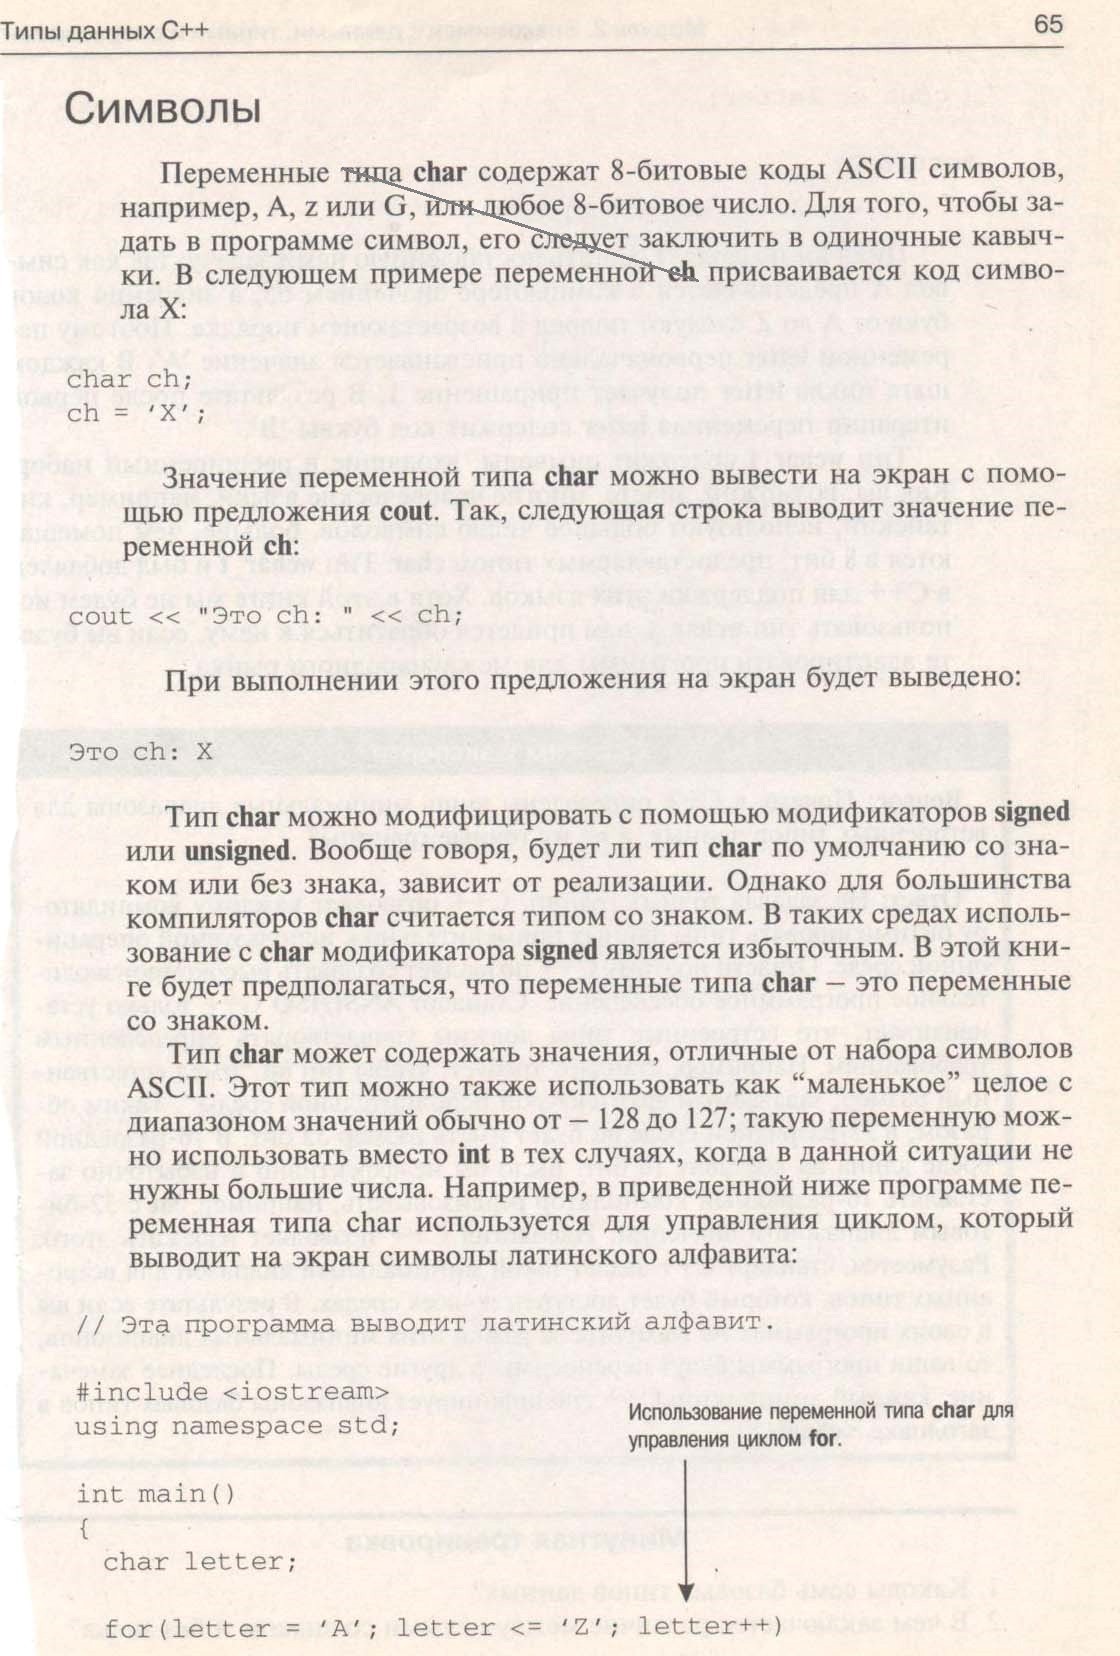
\includegraphics[width=0.7\linewidth]{part-1}
				\caption{Исходное изображение}
				\label{fig:part-1}
			\end{figure*}
			
		Отличительные особенности: структура страницы, использование разных шрифтов, наличие специальных символов, графики (стрелка), внесена погрешность в виде перечеркивания текста линией. Внесенная погрешность немного отличается для каждого из изображений, т.к. линия получалась различной толщины при разных dpi. Однако это не помешало исследовать качество распознавания и не повлияло существенно на количество ошибок распознавания (см. сравнительные таблицы далее).
		
		Распознавание данного изображения производилось в качестве 200, 300, 600  и 100 dpi (точек на дюйм).
		
		Результат распознавания сохранялся в формате *.doc.
		
		\subsubsection{100 dpi}
			
			\begin{figure*}[h]
				\centering
				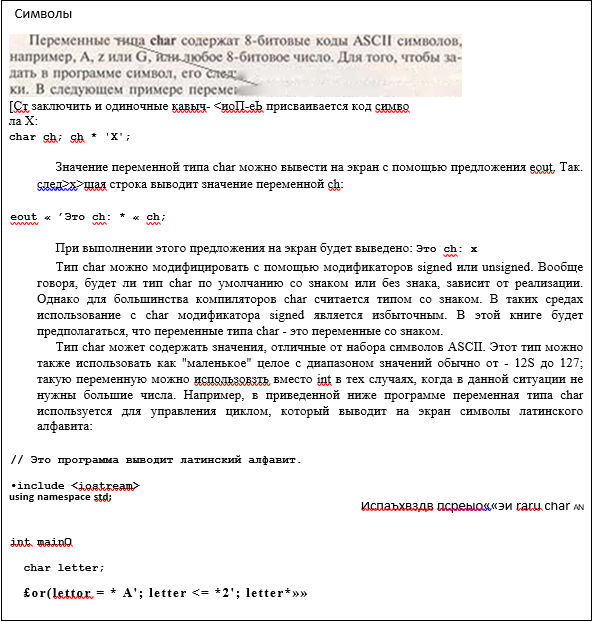
\includegraphics[width=0.7\linewidth]{dpi-75}
				\caption{Результат распознавания изображения 100 dpi}
				\label{fig:dpi-75}
			\end{figure*}
		
		\textbf{Вывод о распознавании:} очень низкое качество, плохое разделение по соответствующим шрифтам. Часть текста с внесенной погрешностью не была распознана вовсе. Однако структура приближенно сохранена. Такой результат, в отличие от всех предыдущих, потребует сильной корректировки человеком. Много слов распознано кардинально неверно.
		
		\subsubsection{200 dpi}
			\begin{figure*}[h]
				\centering
				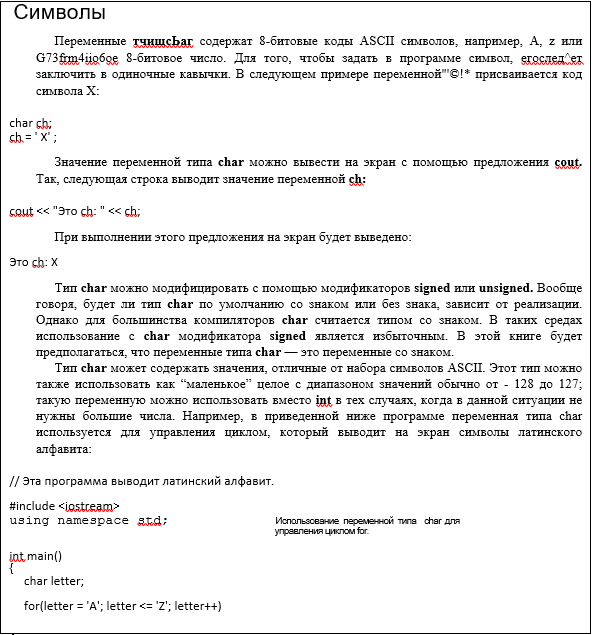
\includegraphics[width=0.7\linewidth]{dpi-200}
				\caption{Результат распознавания изображения 200 dpi}
				\label{fig:dpi-75}
			\end{figure*}
		
		\textbf{Вывод о распознавании:} сохранилась структура, существенных ошибок нет. Разные шрифты. Внесенная погрешность в большинстве мест целиком изменила слово или словосочетание, через которое проходила линия (кроме слова «следует»).

		\subsubsection{300 dpi}
		\begin{figure*}[h]
			\centering
			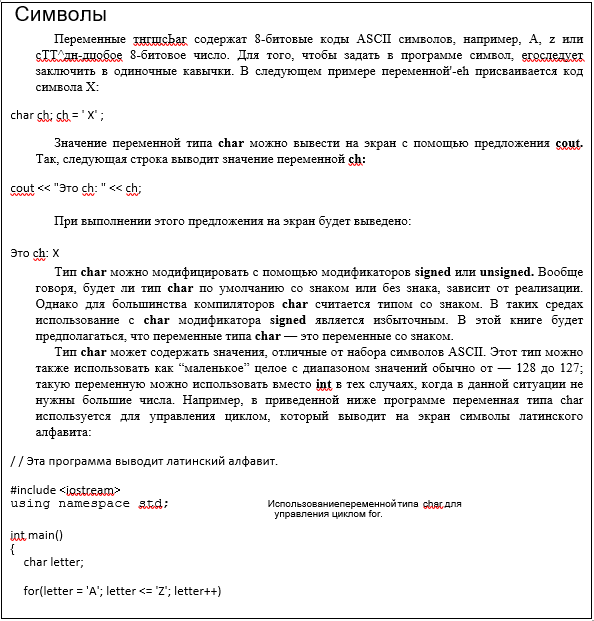
\includegraphics[width=0.7\linewidth]{dpi-300}
			\caption{Результат распознавания изображения 300 dpi}
			\label{fig:dpi-75}
		\end{figure*}
		
		\textbf{Вывод о распознавании:} также сохранилась структура, существенных ошибок нет. Разные шрифты. Однако в некоторых местах исчезли или, наоборот, добавились лишние пробелы, что плохо. Внесенная погрешность в большинстве мест также целиком изменила слово или словосочетание.
		
		\newpage
		\subsubsection{600 dpi}
		\begin{figure*}[h]
			\centering
			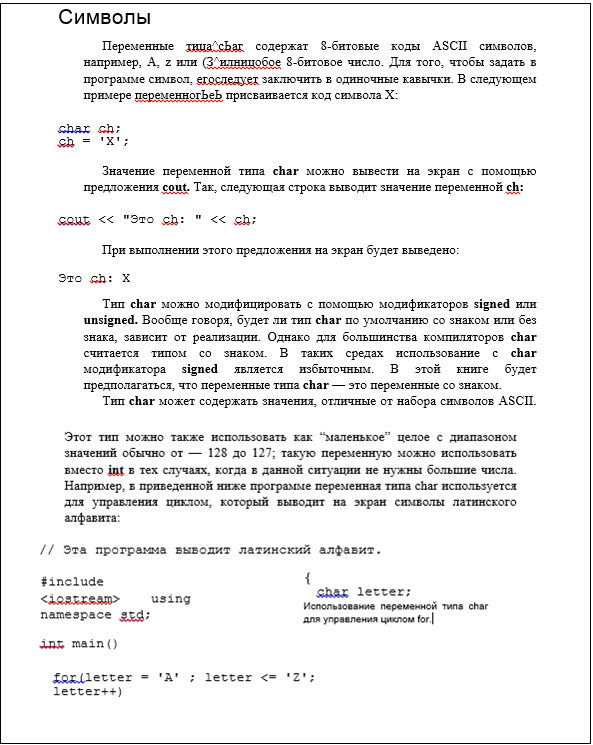
\includegraphics[width=0.7\linewidth]{dpi-600}
			\caption{Результат распознавания изображения 600 dpi}
			\label{fig:dpi-75}
		\end{figure*}
		
		\textbf{Вывод о распознавании:} структура сохранилась, однако в нижней части документа произошел некий сдвиг. Существенных ошибок также нет, шрифты разные. Наилучшее распознавание части текста с внесенной  погрешностью относительно предыдущих случаев.
		
		\begin{tabular}{|c|c|c|}
			\hline
			\multirow{2}{*}{DPI} & \multicolumn{2}{l|}{Количество сомнительных символов} \\ \cline{2-3} 
			& с внесёнными погрешностями & без погрешностей \\ \hline
			100	&     11\% (144/1356)      &   10\% (151/1557)        \\ \hline
			200 &     5\% (83/1585)      &     3\% (50/1584)      \\ \hline
			300 &      6\% (90/1579)     &     4\% (57/1580)      \\ \hline
			600 &     5\% (77/1578)      &     3\% (50/1581)      \\ \hline
		\end{tabular}
	
		\subsubsection{Вывод} Данная программа хорошо подходит для распознавания текстов с различной структурой, размером и шрифтом текста. В результате распознавания получаем документ, который практически не нуждается в дополнительном редактировании человеком. 
		
		При разрешении 200 dpi получаем достаточно высокое качество, такое же получаем при 600. А вот при значении 300 получаем качество хуже. В связи с этим можно сделать вывод, что оптимальным будет значение 200 dpi: оно обеспечивает меньший размер исходного изображения, высокое качество получаемого документа, может исключить ряд ошибок, которые могут возникнуть в результате распознавания погрешностей в исходном изображении (например, клякс) как неких символов.
		
		\subsection{Сравнение качества распознавания нескольких различных изображений с текстом с помощью программ Fine Reader и Free Online OCR.}
		
		Для сравнения возьмем два изображения: первое – слабо структурированное с различными видами текста, 72 точки на дюйм; второе – сильно структурированное (диаграмма UML) с одним видом текста, 96 точек на дюйм. Под видом текста понимается размер текста, шрифт, цвет и т. д.
		
		\subsubsection{Слабо структурированное изображение}
		
			\begin{figure*}[h]
				\centering
				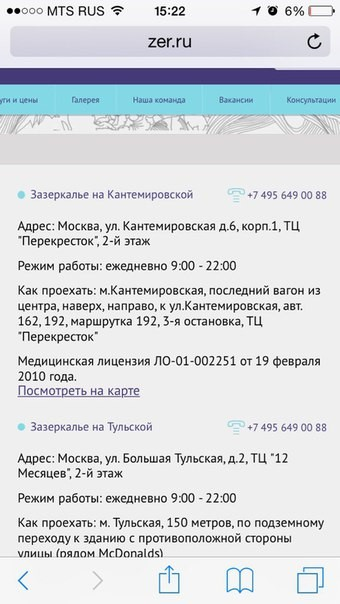
\includegraphics[width=0.5\linewidth]{screen-1}
				\caption{Исходное изображение}
				\label{fig:screen-1}
			\end{figure*}
		
			\begin{figure*}[h]
				\centering
				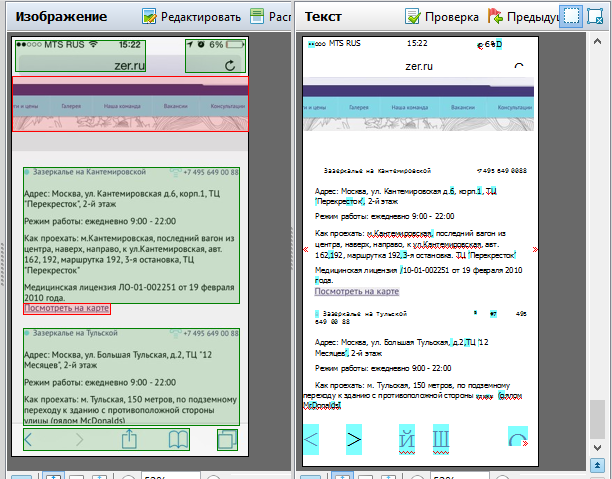
\includegraphics[width=0.7\linewidth]{images/fine-reader-screen}
				\caption{Результат распознавания с помощью FineReader}
				\label{fig:fine-reader-screen}
			\end{figure*}
		
			\begin{figure*}[h]
				\centering
				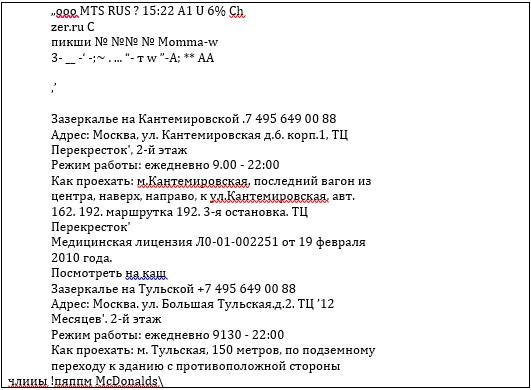
\includegraphics[width=0.7\linewidth]{images/free-online-screen}
				\caption{Результат распознавания с помощью Free Online OCR}
				\label{fig:free-online-screen}
			\end{figure*}
		
		\FloatBarrier
		
		\textbf{FineReader:} есть части, которые распознать не удалось. Структура, в целом, сохранена. Шрифт тоже. Были верно распознаны некоторые специальные символы (например, точки в левом верхнем углу).
		
		\textbf{Free Online OCR:} распознавание именно самого текста хорошее. Однако шрифт стал единым. Структура текста сохранена, но хуже, чем в предыдущем случае. Видно, что возникли проблемы распознавания с теми же частями текста, что и у FineReader-a. Однако часть «Посмотреть на карте» была почти верно распознана. Специальные символы не распознаны (те же самые точки заменены на буквы «о»).
			 	
		\subsubsection{Сильно структурированное изображение}
			\begin{figure*}[h]
				\centering
				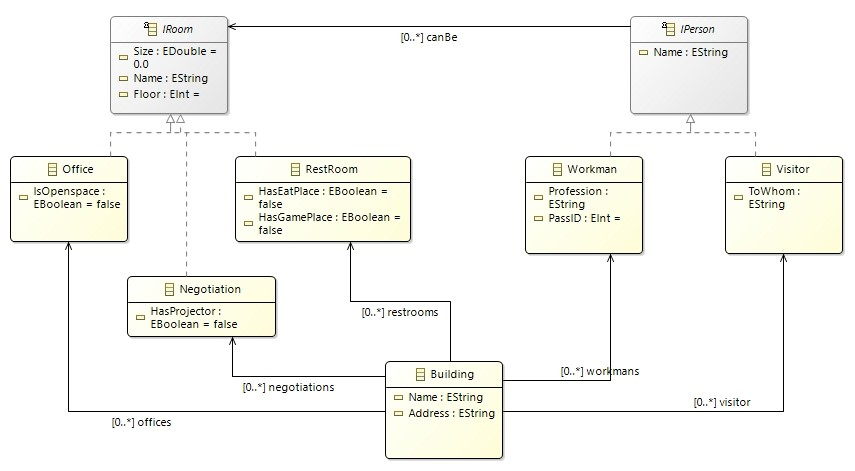
\includegraphics[width=0.7\linewidth]{images/uml}
				\caption{Исходное изображение}
				\label{fig:uml}
			\end{figure*}
			\begin{figure*}[h]
				\centering
				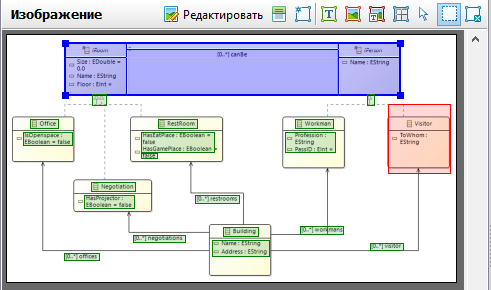
\includegraphics[width=0.7\linewidth]{images/uml-finereader}
				\caption{Результат распознавания с помощью FineReader. Изображение.}
				\label{fig:uml-finereader}
			\end{figure*}
			\begin{figure*}[h]
				\centering
				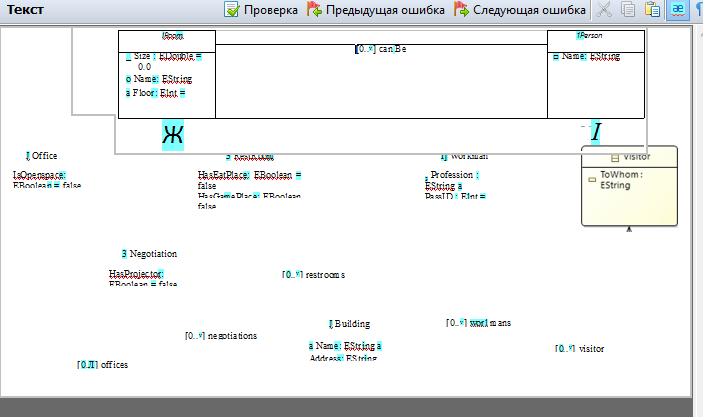
\includegraphics[width=0.7\linewidth]{images/uml-finereader2}
				\caption{Результат распознавания с помощью FineReader. Текст.}
				\label{fig:uml-finereader2}
			\end{figure*}
			\begin{figure*}[h]
				\centering
				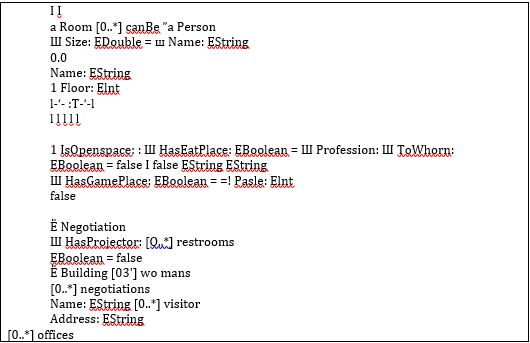
\includegraphics[width=0.7\linewidth]{images/uml-free-ocr}
				\caption{Результат распознавания с помощью Free Online OCR}
				\label{fig:uml-free-ocr}
			\end{figure*}
		
		\FloatBarrier
		
		\textbf{FineReader:} сохранение структуры по блокам. Качество распознавания текста также очень высоко.
		
		\textbf{Free Online OCR:} блочная структура не сохранена, единый шрифт. Качество распознавания текста достаточно хорошее.
		
		\subsubsection{Вывод}
		Безусловно, FineReader обладает весомыми преимуществами по сравнению с Free Online OCR: сохранение даже сложной структуры, размера и шрифта текста, замена нераспознанных частей исходными изображениями, высокое качество распознавания. Однако данная программа имеет платную лицензию, и требует некоторых ресурсов машины для своей работы.
		
		Free Online OCR в свою очередь, может лишь похвастаться хорошим качеством распознавания текста, а также тем, что программа является бесплатной, быстрой и доступна онлайн через интернет, не требуя, соответственно, ресурсов компьютера и являясь мобильной (необходимо лишь только подключение к сети Интернет). Такая программа хорошо подойдет для распознавания сканированных страниц документов в качестве 200 dpi, и практически не потребует дальнейшего редактирования человеком.
		
		\subsection{Сравнение качества распознавания одного изображения текста низкого качества с обучением по шаблону и без него.}
		Данный текст является рукописным. Произведем распознавание данного текста, а затем, также, распознавание с созданием и обучением эталона.
		\begin{figure*}[h]
			\centering
			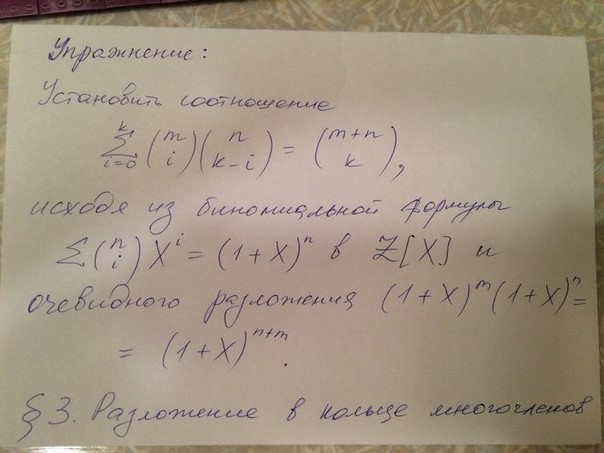
\includegraphics[width=0.7\linewidth]{images/handwrite}
			\caption{Рукописный текст}
			\label{fig:handwrite}
		\end{figure*}
				
		\begin{figure*}[h]
			\centering
			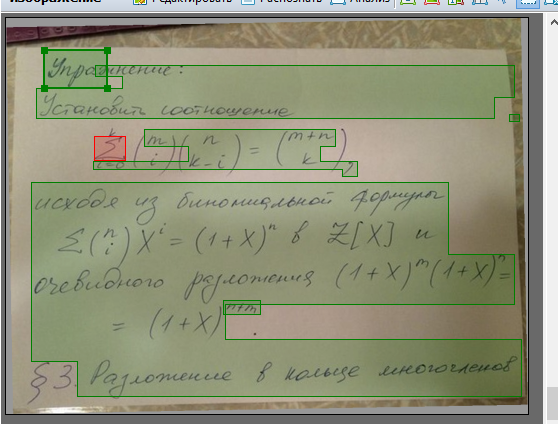
\includegraphics[width=0.7\linewidth]{images/handwrite-no-template}
			\caption{Распознавание текста}
			\label{fig:handwrite-no-template}
		\end{figure*}
		\begin{figure*}[h]
			\centering
			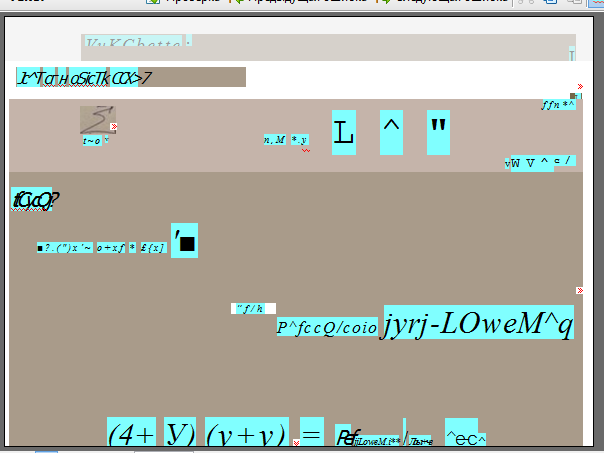
\includegraphics[width=0.7\linewidth]{images/handwrite-no-template2}
			\caption{Результат распознавания текста}
			\label{fig:handwrite-no-template2}
		\end{figure*}
		\begin{figure*}[h]
			\centering
			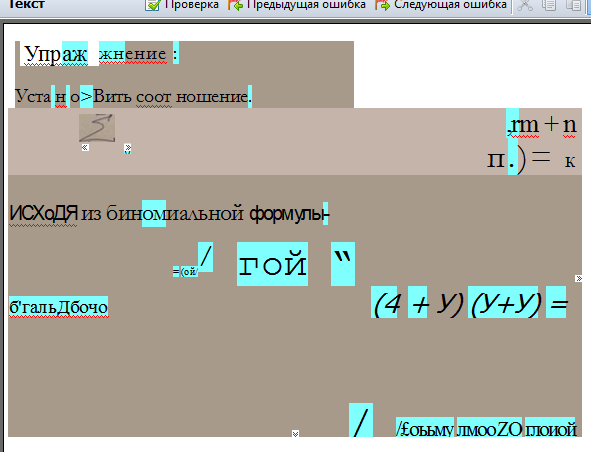
\includegraphics[width=0.7\linewidth]{images/handwrite-with-template}
			\caption{Результат распознавания после процедуры ручного обучения эталона}
			\label{fig:handwrite-with-template}
		\end{figure*}
	
	\FloatBarrier
	
	\subsubsection{Вывод}
		Для рукописного текста обучение помогло программе лучше распознать текст, однако для достаточно точного хорошего распознавания потребуется долгое обучение эталона, а ошибки, связанные с особенностью почерка человека, не будут исключены.
		
		Обучение эталона может помочь для распознавания печатных текстов, где по каким-либо причинам некоторые символы плохо распознаются, а, наверное, наиболее эффективно – для рукописного текста с печатными буквами.
